% Chapter Template

\chapter{Mapping and Scheduling} % Main chapter title

\label{c:sched} % Change X to a consecutive number; for referencing this chapter elsewhere, use \ref{ChapterX}

%----------------------------------------------------------------------------------------
%	SECTION 1
%----------------------------------------------------------------------------------------

The two mode AMC response time analysis for mixed criticality systems was presented in Section~\ref{s:mixedcriticality}. We have shown that it is advantageous to consider a four mode model when both transient faults and execution time ovearruns are possible in a single lockstep-core mixed criticality fault tolerant system (MCFTS) \cite{albayati2016modes}. This chapter will review the four mode analysis and then extend it to include several ODR strategies in multicore systems. A DSE mapping algorithm that uses the new analysis will then be presented which is similar to \cite{bolchini2013reliability} and \cite{kang2014reliability}.

\section{Four Mode Response Time Analysis for MCFTS}

	The motivation for four modes in a MCFTS is to reduce the number of LO tasks that must be dropped in the event that only an execution overrun or transient fault occurs rather than both. 
	We initially consider a lockstep core that is capable of detecting but not correcting errors.
	The RTOS kernel is assumed to remain uncorrupted.
	Under these conditions, a task may be re-executed when an error is detected.
	\addfigure{0.6}{modes.pdf}{The 4 modes of operation in MCFTS analysis.}{f:modes}
\addfigure{0.6}{sched-example.pdf}{Mode change scenarios.}{f:mode-scenarios}
	
	The four modes and their transition conditions are shown in Figure~\ref{f:modes}. 
	Furthermore, three possible scenarios are presented in Figure~\ref{f:mode-scenarios} for the task set in Table~\ref{t:example}.
	In scenario (a), $\tau_1$ exceeds its $C(LO)$ threshold of 3 and the system transitions into OV mode. In scenario (b), $\tau_1$ suffers a transient fault and required re-execution. The system stays in TF mode because none of the re-executions exceed $C(LO)$. In scenario (c), $\tau_1$ first exceeds $C(LO)$ and the system transitions to OV mode. Once in OV mode, an fault occurs and the system transitions into HI mode, presumably dropping even more tasks.
	
	
	
\section{}
	
	
	\begin{table}[t!]
\caption{Example Task Set}
\centering

	\begin{tabular}{@{}lcccc@{}}
	\toprule
	& $C(LO)$ & $C(HI)$ & T=D & L 	 \\
	\bottomrule
	$\tau_1$ & 3 & 4 & 12 & HI  \\
	$\tau_2$ & 4 & - & 12 & LO  \\
	$\tau_3$ & 4 & - & 12 & LO  \\
	$\tau_4$ & 1 & - & 12 & LO  \\
	\end{tabular}

\label{t:example}
\end{table}
	
	%In addition to the LO and HI modes, there is now a transient fault (TF) and overrun (OV) mode. 
	Equations \ref{eq:lomode}-\ref{eq:hiovmode} show the updated response time analysis.
	
	
\begin{equation}
R_i^{(LO)}= C_i(LO)+\sum_{j \in hp(i)}\Big\lceil\frac{R_i^{(LO)}}{T_j}\Big\rceil \cdot C_j(LO)
\label{eq:lomode}
\end{equation}

\begin{equation}\label{eq:ovmode}
\begin{aligned}
R_i^{(OV)} &  = C_i(L_i)+\sum_{j \in hpC(OV,i)}\Big\lceil\frac{R_i^{(OV)}}{T_j}\Big\rceil \cdot C_j(L_j) 
 +\sum_{k \in hp(i)-hpC(OV,i)}\Big\lceil\frac{R_i^{(LO)}}{T_k}\Big\rceil \cdot C_k(LO)
\end{aligned}
\end{equation}
	
	
	The LO mode analysis remains unchanged. Equation~\ref{eq:ovmode} shows the response time for the OV mode. 
	The set of tasks $hpC(L,i)$ is defined as the set of tasks with higher priority than $\tau_i$ that are not dropped in mode $L$. 
	Therefore, in the OV mode, we can see that the jobs that continue to execute are assumed to take the maximum amount of time $C(OV)=C(HI)$ whereas the dropped jobs ($hp(i) - hpC(OV,i)$) only execute during $R_i(LO)$ for up to their $C(LO)$ times.
	
\begin{equation}\label{eq:tfmode}
\begin{aligned}
R_i^{(TF)} & = n_i(TF) \cdot C_i(LO)
+\sum_{j \in hpC(TF,i)}\Big\lceil\frac{R_i^{(TF)}}{T_j}\Big\rceil \cdot n_j(TF) \cdot C_j(LO) \\
&  +\sum_{k \in hp(i)-hpC(TF,i)}\Big\lceil\frac{R_i^{(LO)}}{T_k}\Big\rceil \cdot C_k(LO)
\end{aligned}
\end{equation}

	Equation~\ref{eq:tfmode} shows the response time for TF mode. 
	In the transient fault mode at least one task must re-execute. 
	Each task is assigned a maximum number of executions that it is required to run, $n_i$, in order to meet some threshold in terms of probability of failure (derivation in \cite{albayati2016modes}). 
	In the TF mode, the execution time is still assumed not to exceed the optimistic threshold $C(LO)$. 
	The resulting execution time for task $\tau_i$ is $n_i(TF) \cdot C_i(LO)$ where $n_i$ is the number of re-executions required in the TF mode.\footnote{$n$ depends on $C$, therefore it is possible that $n(TF) \ne n(HI)$ though this is not often the case.}

	Finally, Equations~\ref{eq:hiovmode} and \ref{eq:hitfmode} show the response time analysis for transitions from OV to HI and TF to HI modes, respectively. The set of dropped jobs on the final transition is different for the two modes.





\begin{equation}\label{eq:hiovmode}
\begin{aligned}
R_i^{(HI-OV)} & = n_i(HI) \cdot C_i(L_i) 
  +\sum_{j \in hpC(HI,i)}\Big\lceil\frac{R_i^{(HI-OV)}}{T_j}\Big\rceil \cdot n_j(HI) \cdot C_j(L_j) \\
&  +\sum_{k \in hpC(OV,i)-hpC(HI,i)}\Big\lceil\frac{R_i^{(OV)}}{T_k}\Big\rceil \cdot C_k(LO) \\
& \hspace{1cm}  +\sum_{l \in hp(i)-hpC(OV,i)}\Big\lceil\frac{R_i^{(LO)}}{T_l}\Big\rceil \cdot C_l(LO)
\end{aligned}
\end{equation}

\begin{equation}\label{eq:hitfmode}
\begin{aligned}
R_i^{(HI-TF)} & = n_i(HI) \cdot C_i(L_i)
  +\sum_{j \in hpC(HI,i)}\Big\lceil\frac{R_i^{(HI-TF)}}{T_j}\Big\rceil \cdot n_j(HI) \cdot C_j(L_j) \\
&  +\sum_{k \in hpC(TF,i)-hpC(HI,i)}\Big\lceil\frac{R_i^{(TF)}}{T_k}\Big\rceil \cdot C_k(LO) \\
& \hspace{1cm}  +\sum_{l \in hp(i)-hpC(TF,i)}\Big\lceil\frac{R_i^{(LO)}}{T_l}\Big\rceil \cdot C_l(LO)
\end{aligned}
\end{equation}




\section{Extending Response Time Analysis to ODR}

	We will extend the analysis on lockstep (LS) to support three types of ODR. The four scenarios are shown in Figure~\ref{f:ftm}. 
	In (a), LS execution occurs when a node has internal mechanisms for detecting but not correcting errors. 
	An error simply results in a re-execution on that node, as previously discussed. 	
	In (b), dual modular redundancy (DMR) replicates a thread on two cores that cannot detect errors. 
	The task must be re-executed if the task executions are found not to match by some external comparison and voting mechanism.
	In (c), triple modular redundancy (TMR) replicates a thread on three cores that cannot detect errors. 
	If an error occurs, the majority answer is taken from the three replicas and no re-execution is required.
	Finally, in (d), passive replication is similar to TMR but the final replica does not execute if the first two copies return the same result. 


\addfigure{0.55}{ftm.pdf}{The 4 fault tolerance mechanisms supported by the proposed MCFTS analysis}{f:ftm}
	
	Each technique is expressed in the new analysis by three parameters: a task set transformation, mapping constraints, and a re-executiong profile denoted by $N$.
	The task set transformation represents each replica explicitly in the task set. 
	Consider the example task set in Table~\ref{t:transform}. 
	Lockstep does not introduce any replicas to the system and does not require any transformation of the task set. 
	DMR requires one replica to be added to the task set while TMR and PR require two replicas to be added.
	
	Constraints must be added to the problem for the processors $\pi_i$ assigned to $\tau_i$ in order to properly reflect the semantics of the different techniques. 
	The constraints shown in the table ensure that the replicas are not assigned to the same core. 
	These constraints will be useful in the mapping stage.
	
	
\begin{table}
\centering
\caption{Task set transformations}
\label{t:transform}
	\begin{subtable}{0.3\textwidth}
		\caption{Example task set}
		\begin{tabular}{@{}l|cccc@{}}
		\toprule
		& C(LO) & C(HI) & T=D & L 	 \\\bottomrule
		$\tau_1$ & 5 & 10 & 25 & HI  \\
		$\tau_2$ & 5 & - & 20 & LO  \\
		\multicolumn{5}{c}{ } \\
		\multicolumn{5}{c}{ } \\
		\end{tabular}
	\end{subtable} \hspace{2cm}
	\begin{subtable}{0.3\textwidth}
		\caption{DMR transformation}
		\begin{tabular}{@{}l|cccc@{}}
		\toprule
				& C(LO) & C(HI) & T=D & L	 \\\bottomrule
		$\tau_1$ & 5 & 10 & 25 & HI  \\
		$\tau_{1.1}$ & 5 & 10 & 25 & HI  \\
		$\tau_2$ & 5 & - & 20 & LO  \\
		\multicolumn{5}{c}{$\pi_1 \ne \pi_{1.1}$}
		\end{tabular}
	\end{subtable}
	
	\begin{subtable}{0.3\textwidth}
		\caption{TMR transformation}
		\begin{tabular}{@{}l|cccc@{}}
		\toprule
				& C(LO) & C(HI) & T=D & L	 \\\bottomrule
		$\tau_1$ & 5 & 10 & 25 & HI  \\
		$\tau_{1.1}$ & 5 & 10 & 25 & HI  \\
		$\tau_{1.2}$ & 5 & 10 & 25 & HI  \\
		$\tau_2$ & 5 & - & 20 & LO  \\
		\multicolumn{5}{c}{$\pi_1 \ne \pi_{1.1} \ne \pi_{1.2}$}
		\end{tabular}
	\end{subtable} \hspace{2cm}
	\begin{subtable}{0.3\textwidth}
		\caption{PR replication}
		\begin{tabular}{@{}l|cccc@{}}
		\toprule
		& C(LO) & C(HI) & T=D & L	 \\\bottomrule
		$\tau_1$ & 5 & 10 & 25 & HI  \\
		$\tau_{1.1}$ & 5 & 10 & 25 & HI  \\
		$\tau_{1.2}$ & 5 & 10 & 25 & HI  \\
		$\tau_2$ & 5 & - & 20 & LO  \\
		\multicolumn{5}{c}{$\pi_1 \ne \pi_{1.1}$}
		\end{tabular}
	\end{subtable}
\end{table}


	The re-execution variable $n_i$ has been generalized into the vector:
\begin{equation}
	N_i=<n_i(LO),n_i(OV),n_i(TF),n_i(HI)>
\end{equation} 
	The $N$ for each mode is shown in Table~\ref{t:reex} and the updated equation for the OV mode response time are given by the following equations:
	\begin{equation}
\begin{aligned}
R_i^{(OV)} =
\begin{dcases*}
C_i(L_i)\color{red} \color{black}+\sum_{j \in hpC(OV,i)}\Big\lceil\frac{R_i^{(OV)}}{T_j}\Big\rceil \cdot C_j(L_j) \\
\hspace{0.3cm} +\sum_{k \in hp(i)-hpC(OV,i)}\Big\lceil\frac{R_i^{(LO)}}{T_k}\Big\rceil \cdot C_k(LO), &  $n_i(OV)>0$ \\
	0, & $n_i(OV)=0$
\end{dcases*}
   \end{aligned}
\end{equation}
	We note that all techniques have $n(LO)$ and $n(OV)$ values of either 0 or 1. When $n=0$, the task is not executing and the response time is simply 0. The same is true for LO mode.
	
	For example, TMR has $N=<1,1,1,1>$. This means that in all modes, any task using TMR will have $n=1$ which in effect signals that no re-executions are required. For PR, one replica executes one time in all modes and the other only executes in the case of a fault (hence only executes once in TF or HI modes).

	\begin{table}
\caption{Re-execution profiles for the fault tolerance mechanisms}
\label{t:reex}
\centering
	\begin{tabular}{@{}l|c@{}}
	\toprule
	Technique & Profile ($N$) \\
	\bottomrule
	LS & $<1,2,1,2>$ \\
	DMR & $<1,2,1,2>$ \\
	TMR & $<1,1,1,1>$ \\
	PR & $<1,1,1,1>$ and $<0,1,0,1>$ \\
	\end{tabular}
\end{table} 	

\section{Design Space Exploration}

\subsection{Genetic Algorithm}

\subsection{Two Stage GA}
	The mapping and scheduling algorithm follows the procedure used in \cite{bolchini2013reliability} and \cite{kang2014reliability}. Two stages of genetic algorithms (GA) are used to explore both the techniques used to harden each task and the core assignment for each task and its replicas. The basic flow is shown in Figure~\ref{f:dse}. The Reliability Aware (RA) stage is responsible for assigning 
	
\addfigure{0.6}{dse.pdf}{Overview of DSE workflow using nested genetic algorithm searches}{f:dse}
	
	

% The initial scheduling algorithm will be taken from Bolchini and  Miele \cite{bolchini2013reliability}. A genetic algorithm (GA) is used to explore the design space. The general details that follow on genetic algorithms are based on the overview in \cite{geatbx}.
% 
% Figure \ref{f:ga_ov} shows an overview of how to implement a genetic algorithm. There are two stages of GA in the given process. First tasks must be organized into groups of tasks, and each group of tasks must be assigned a fault detection technique or fault tolerance technique. DMR Fingerprinting is an example of a detection mechanism. This work will remain agnostic about the method of implementation of fault tolerance. We assume that appropriate hardening measures are applied to a single core.
%  
% \begin{figure}[h]
% \centering
% 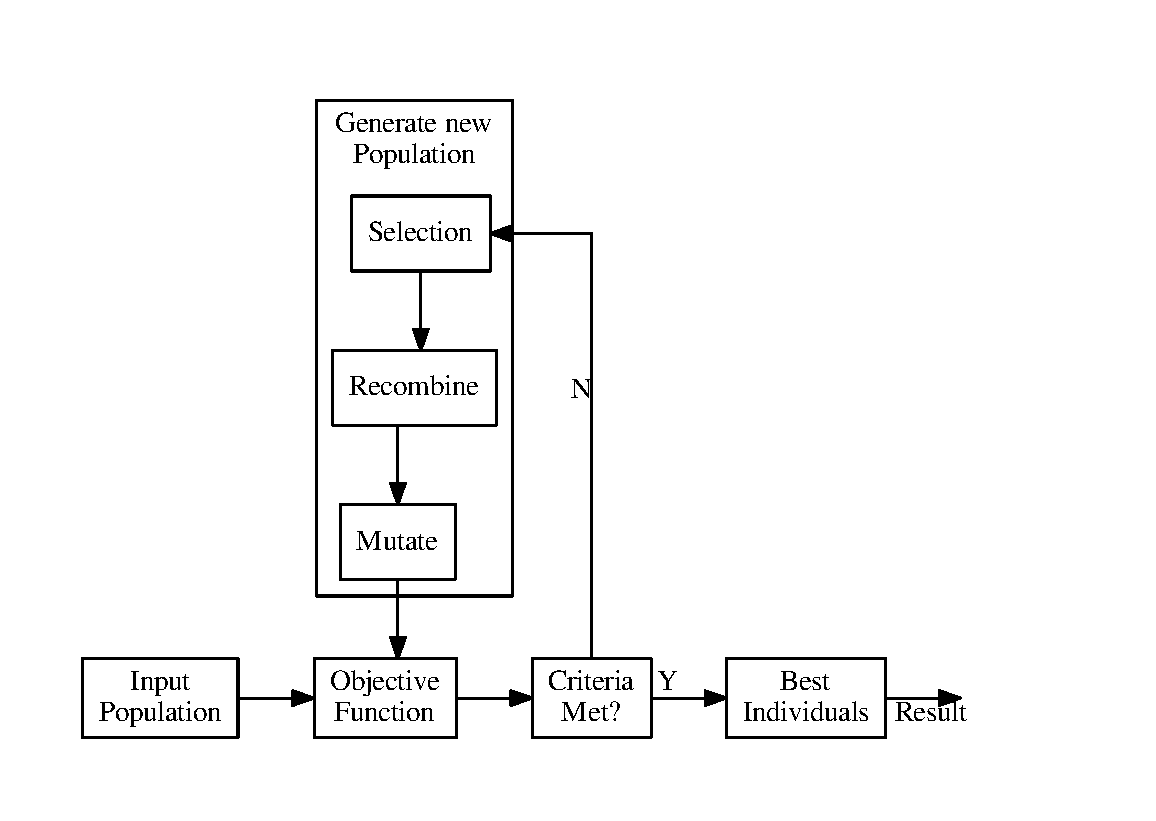
\includegraphics[width=12cm]{ga_ov}
% \caption{The basic structure of a genetic algorithm \cite{geatbx}.} 
% \label{f:ga_ov}
% \end{figure}
% 
% Once a population of various groupings and associated fault-handling mechanisms has been generated it is necessary to test their fitness. This must be done by generating a system schedule for each member of the population. 
% 
% The generation of the schedule is itself done with a second round of GA. Each task is assigned to an appropriate core based on the fault-handling requirements of its group. The group adopts the most stringent requirements of any of its members. Various mappings are generated as the GA population. Then it is necessary to order the tasks on each core. This is complicated by the fact that there may be inter-core data dependencies. For now, we will neglect the overhead associated with data transfer between cores.
% 
% The implementation details of the genetic algorithm will be adopted from \cite{bolchini2013reliability}. Tournament selection and single-point crossover operator recombination will be used. Mutations will be applied randomly. There are four mutations at the task level: change the group of a task, split a group in two, join two groups, or change the fault-management technique applied to a group. The mutation for the mapping phase consists of switching a task to another processor that can meet the assigned fault-management requirements.
% 
% Tournament selection means choosing a subset of the population and selecting the most fit member. This is repeated as many times as necessary. Single-point crossover cuts two parent chromosomes into two pieces and then exchanges the second substrings between the chromosomes. 
% 
% The initial parameters for the GA will be the ones suggested in \cite{bolchini2010multi}. The crossover rate is 80\%, the mutation rate is 10\%. The program will run for 30 generations. The population size will be between one and two thousand.
% 
% The JGAP library \cite{jgap} is used to implement the genetic algorithm. 



